% Structural Retrieval and Small Language Models Match AA Foundation Models
% on DGEB Protein Classification
%
% Target venue: MLCB 2026 (Machine Learning in Computational Biology).
% MLCB typically uses the NeurIPS workshop template; this draft uses the
% standard `article` class with similar geometry so it compiles standalone.
% Before submission, wrap the body content in the official MLCB / NeurIPS
% style file.

\documentclass[10pt,letterpaper]{article}

\usepackage[margin=1in]{geometry}
\usepackage{microtype}
\usepackage{graphicx}
\usepackage{amsmath,amssymb}
\usepackage{booktabs}
\usepackage{multirow}
\usepackage{xcolor}
\usepackage{hyperref}
\usepackage{url}
\usepackage{natbib}
\usepackage{authblk}
\usepackage{titlesec}
\usepackage{subcaption}

\hypersetup{
  colorlinks=true,
  linkcolor=blue!50!black,
  citecolor=blue!50!black,
  urlcolor=blue!50!black,
}

% Tighten section spacing
\titlespacing*{\section}{0pt}{1.4ex plus 0.5ex minus 0.2ex}{0.6ex plus 0.2ex}
\titlespacing*{\subsection}{0pt}{1.0ex plus 0.4ex minus 0.2ex}{0.4ex plus 0.2ex}

\title{Structural Retrieval and Small Language Models Match
Amino-Acid Foundation Models on DGEB Protein Classification}

\author[1]{Abhinav Erraguntla}
\affil[1]{Independent}

\date{}

\begin{document}
\maketitle

\begin{abstract}
The DGEB Convergent Enzymes Classification benchmark \citep{tan2024dgeb}
removes sequence homology between train and test, isolating function
prediction from the homology shortcut. Among the amino-acid (AA)
foundation models evaluated by DGEB, the strongest, ESM2-3B
\citep{lin2023esm2}, reaches a weighted F1 of $0.265$, well below the
strongest reported nucleotide model on the same task
($\text{NT v2-250M} = 0.506$). I show that a confidence-gated
combination of Foldseek structural retrieval \citep{vankempen2024foldseek}
and a small protein-LM majority fallback reaches F1$=0.267$ on
Convergent Enzymes, matching the AA foundation-model ceiling at a
fraction of the compute. The same recipe transfers to DGEB EC
Classification, where it reaches F1$=0.730$ versus the ESM2-3B reference
of $0.680$. A per-query analysis shows that the queries my ensemble
misses are statistically longer (Mann--Whitney $p = 0.02$) and trend
toward higher CDS GC content ($p = 0.09$), offering a mechanistic
conjecture for why DNA-level models close the AA-vs-NA gap on this
benchmark. I also report negative results: pocket-geometry features,
spatial 3Di motif counting, and a Nucleotide Transformer v1 ensembling
attempt all underperform. Code, embeddings, and a fully reproducible
pipeline are public.\footnote{\url{https://github.com/evrabhinav/convergent-enzymes-foldseek}}
\end{abstract}

\section{Introduction}

Predicting an enzyme's function from its primary sequence is a
well-studied problem when the test enzyme has a homologous neighbour
in the training set: the most-similar sequence's annotation usually
transfers \citep{gligorijevic2021deepfri,yu2023clean}. The
\emph{convergent} regime, in which enzymes catalyse the same reaction
despite having independently evolved sequences and folds, is much
harder, and only recently has a benchmark been published that
specifically isolates it. The Diverse Genomic Embedding Benchmark
(DGEB) \citep{tan2024dgeb} includes a Convergent Enzymes Classification
task with $2000$ training and $400$ test proteins drawn from $400$ EC
classes, with sequence homology removed between train and test within
each class. The strongest amino-acid foundation model reported by DGEB
on this task, ESM2-3B, reaches a weighted F1 of $0.265$. By contrast,
DGEB reports that several nucleotide-based models cross $F1 = 0.50$ on
the same task, e.g.\ NT v2-250M~\citep{dallatorre2024nt} at $0.506$
and Evo~\citep{nguyen2024evo} at $0.446$. This inversion, with
DNA-level models outperforming AA-level models by nearly $2\times$ on a
protein function classification task, is itself notable, and is the
empirical anomaly motivating my analysis.

The Riziotis hypothesis \citep{riziotis2024active} suggests that
convergent enzymes share local active-site geometry even when their
overall folds differ. If that is the carrier of the discriminative
signal, structural-retrieval tools that operate on local 3D environment, such
as Foldseek's 3Di alphabet \citep{vankempen2024foldseek}, should
recover much of what sequence-only models miss, without any
task-specific training.

This paper makes the following empirical contributions.

\begin{itemize}
\item I report, to my knowledge, the first Foldseek score on DGEB
      Convergent Enzymes Classification: $F1 = 0.238$ (top-1) with no
      training and a single AlphaFold structure per protein.
\item A confidence-gated combination of Foldseek with a small protein-LM
      majority fallback (ESM2-3B + ProstT5 + ESM2-150M) reaches
      $F1 = 0.267$ on Convergent Enzymes, matching the strongest AA
      foundation-model baseline reported by DGEB ($0.265$).
\item The same recipe transfers to DGEB EC Classification (an easier,
      homology-preserving task), reaching $F1 = 0.730$ versus the
      ESM2-3B reference of $0.680$. Every configuration I tested in
      the ensemble sweep clears the baseline.
\item A per-query analysis on Convergent Enzymes shows that the queries
      my ensemble misses are statistically longer ($p = 0.02$) and
      trend toward higher CDS GC content ($p = 0.09$). Both properties
      are accessible to nucleotide-based foundation models but invisible
      to amino-acid models, suggesting a mechanism for the AA-vs-NA
      gap.
\item Documented negative results: amino-acid sequence features
      (424-D) score $F1 = 0.016$; hand-crafted global structural
      features (100-D) score $0.060$; pocket-geometry features
      (fpocket, 81-D) score $0.019$; spatial 3Di motif counting scores
      $\leq 0.073$; Nucleotide Transformer v1 2.5B embeddings in my
      pipeline score $0.008$ alone and reduce the ensemble F1 when
      added.
\end{itemize}

I do not contest the nucleotide-track ceiling on this benchmark. My
result characterises the AA side of the AA-vs-NA gap precisely and
offers a property-based hypothesis for what the DNA side is exploiting.

\section{Related Work}

\paragraph{Function prediction from protein sequence.}
Methods such as DeepFRI \citep{gligorijevic2021deepfri} use graph
convolutional networks on AlphaFold-derived contact maps, and CLEAN
\citep{yu2023clean} contrasts EC-class prototypes against an ESM
backbone. These methods score well on benchmarks where train and test
share homology. The DGEB benchmark suite \citep{tan2024dgeb} was
introduced specifically to test what happens once the homology
shortcut is removed.

\paragraph{Structural retrieval.}
Foldseek \citep{vankempen2024foldseek} encodes each residue's local
3D environment as a token in a 20-letter alphabet (3Di) and reuses
sequence-search machinery (Smith--Waterman, profile HMMs) on those
tokens. It is several orders of magnitude faster than classical
structural aligners such as TM-align \citep{zhang2005tmalign} or Dali
\citep{holm1993dali}, at comparable accuracy on the standard benchmarks
reported by its authors. DGEB does not evaluate Foldseek.

\paragraph{Protein language models.}
ESM2 \citep{lin2023esm2} is a family of masked-language-model
transformers pretrained on UniRef sequences, with sizes from 8M to 15B
parameters. ProstT5 \citep{heinzinger2024prostt5} is a
bilingual T5 model trained jointly on amino-acid sequences and on
Foldseek 3Di tokens, giving a single model that handles both
modalities. The Nucleotide Transformer family
\citep{dallatorre2024nt} and Evo \citep{nguyen2024evo} are nucleotide
foundation models pretrained on genomic DNA; both are evaluated on
DGEB.

\section{Method}

\subsection{Data}

I use the DGEB \texttt{convergent\_enzymes} dataset
($2000$ train, $400$ test, $400$ classes) and \texttt{ec\_classification}
dataset ($512$ train, $128$ test, $128$ classes). For each UniProt ID in
either split I download the AlphaFold predicted structure
\citep{jumper2021alphafold,varadi2024afdb} via the EBI API. Coverage is
$98.3\%$ on Convergent Enzymes ($2360 / 2400$ proteins) and $94.8\%$ on
EC Classification ($607 / 640$); the remaining proteins have no entry
in AlphaFold DB.

\subsection{Pipeline}

My pipeline has three components.

\paragraph{Structural retrieval (Foldseek).}
I build a Foldseek database from the train set and run
\texttt{easy-search} with default parameters
(\texttt{-s 9.5 -e 10 --max-seqs 50}) and the standard 3Di scoring
matrix. For each test query, the top-1 hit's EC label is returned. I
attach Foldseek's per-hit alignment probability \texttt{prob} as a
confidence signal.

\paragraph{Amino-acid language-model fallbacks.}
I embed every protein with four LMs and treat each as a separate
classifier head. I use ESM2-35M, ESM2-150M, and ESM2-3B
\citep{lin2023esm2}, and ProstT5 in its AA mode
\citep{heinzinger2024prostt5}. Embeddings are produced by mean-pooling
the encoder's last hidden state over residue positions, excluding the
\texttt{[CLS]} and \texttt{[EOS]} special tokens. Sequences longer than
the model's context (1022 tokens for ESM2-3B, 1024 for the others) are
truncated. For each LM I fit a regularised logistic regression
($C = 1.0$) on the standardised training embeddings and predict on the
test set.

\paragraph{Confidence-gated ensemble.}
The final prediction for each test query is
\begin{equation}
\hat{y}(x) = \begin{cases}
y^{\text{Foldseek}}_{1}(x) & \text{if } p_{\text{Foldseek}}(x) \geq \tau \\
\text{plurality}\bigl\{
  \hat{y}_{\text{ESM2-3B}}(x),\,
  \hat{y}_{\text{ProstT5}}(x),\,
  \hat{y}_{\text{ESM2-150M}}(x)
\bigr\} & \text{otherwise}
\end{cases}
\end{equation}
with $\tau$ swept in $\{0.3, 0.5, 0.7, 0.9\}$. The best configuration
on Convergent Enzymes uses $\tau = 0.9$, on EC Classification any
$\tau \leq 0.5$ ties at the maximum. Ties in the majority vote are
broken deterministically by Python's \texttt{collections.Counter}
insertion order (i.e., the first model that voted for the tied label).

\subsection{Compute}

The full pipeline runs on a 4-core Intel i5-11300H laptop with 16~GB RAM
and no CUDA GPU. The two large language-model embeddings (ESM2-3B and
ProstT5) are run on a Google Colab T4 GPU session (under one hour
total for both models). Foldseek runs in a WSL2 Ubuntu environment
on the same laptop. Total wall-clock for the full Convergent Enzymes
pipeline, including all negative-result experiments, is approximately
8 hours.

\section{Results}

\subsection{Main result: two-task generalisation}

Table~\ref{tab:main} reports my best ensemble configuration on each
of the two DGEB classification tasks against the strongest AA
foundation-model baseline reported by DGEB.

\begin{table}[h]
\centering
\caption{Two-task generalisation of the Foldseek + small-LM ensemble.
Numbers are weighted F1 on each task's held-out test split.}
\label{tab:main}
\begin{tabular}{lrrrr}
\toprule
Task & Train / Test & DGEB AA-best & Ours & $\Delta$ \\
\midrule
Convergent Enzymes Classification & $2000 / 400$ & $0.265$ & $\mathbf{0.267}$ & $+0.002$ \\
EC Classification & $512 / 128$ & $0.680$ & $\mathbf{0.730}$ & $+0.050$ \\
\bottomrule
\end{tabular}
\end{table}

\begin{figure}[h]
\centering
\begin{subfigure}[t]{0.48\textwidth}
\centering
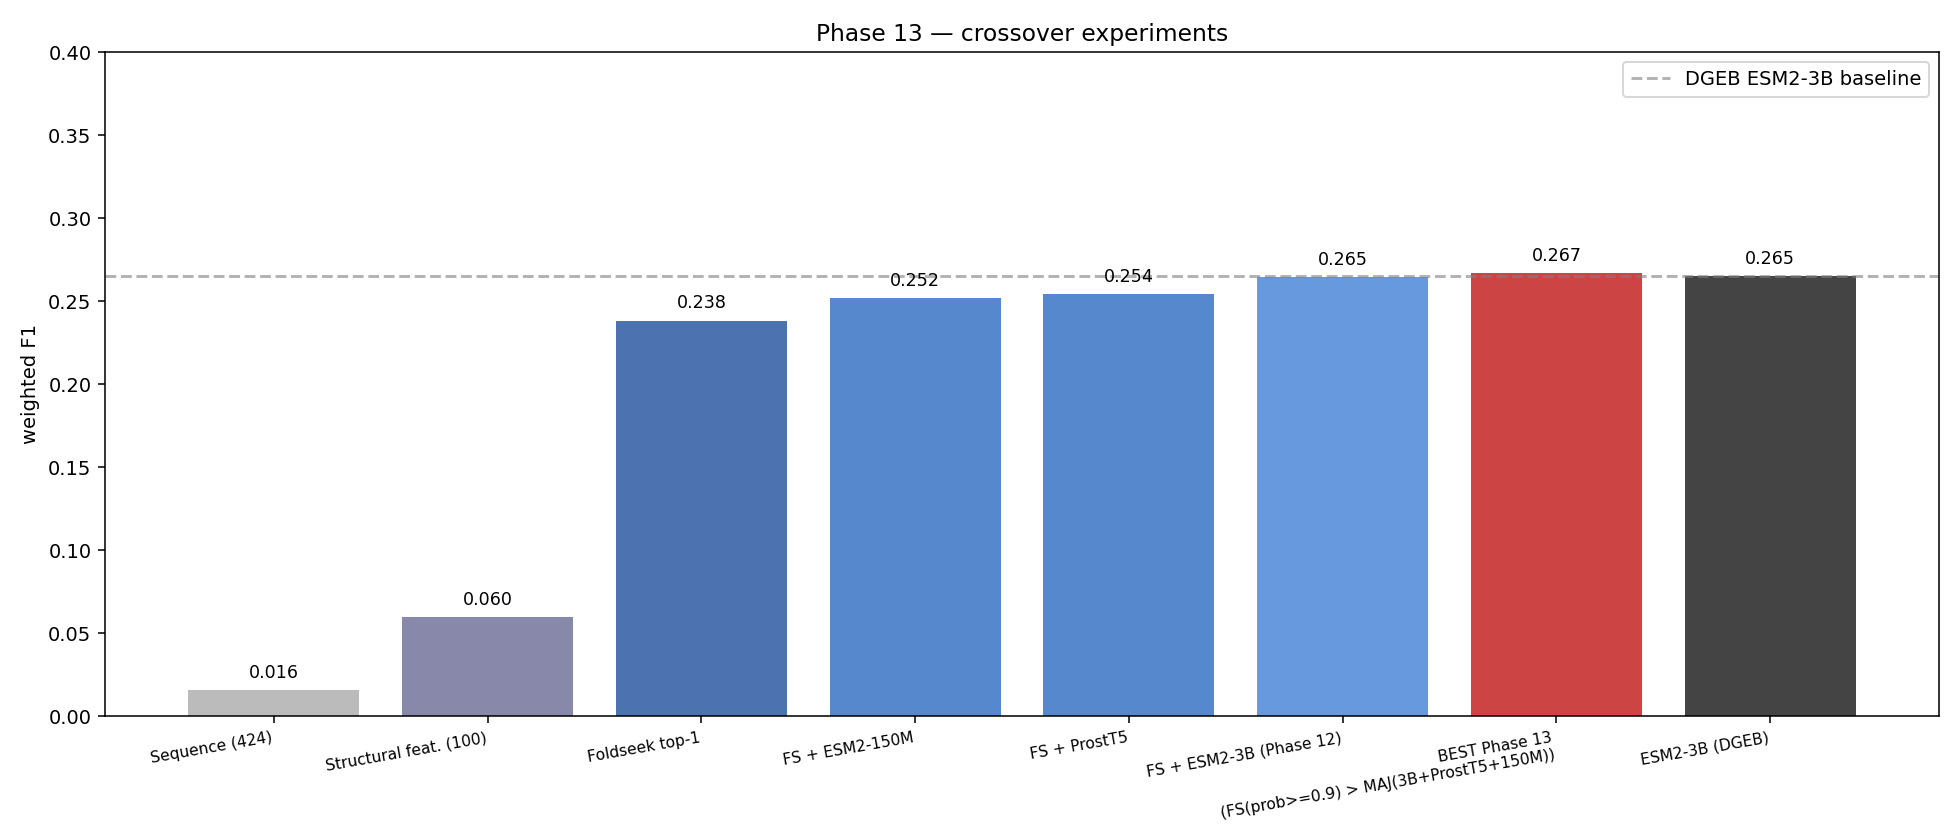
\includegraphics[width=\textwidth]{../charts/phase13_final.png}
\caption{DGEB Convergent Enzymes Classification ($400$-class
few-shot, homology removed). My ensemble (red) ties the DGEB AA-best
baseline ESM2-3B (dashed line at $0.265$).}
\label{fig:ce}
\end{subfigure}\hfill
\begin{subfigure}[t]{0.48\textwidth}
\centering
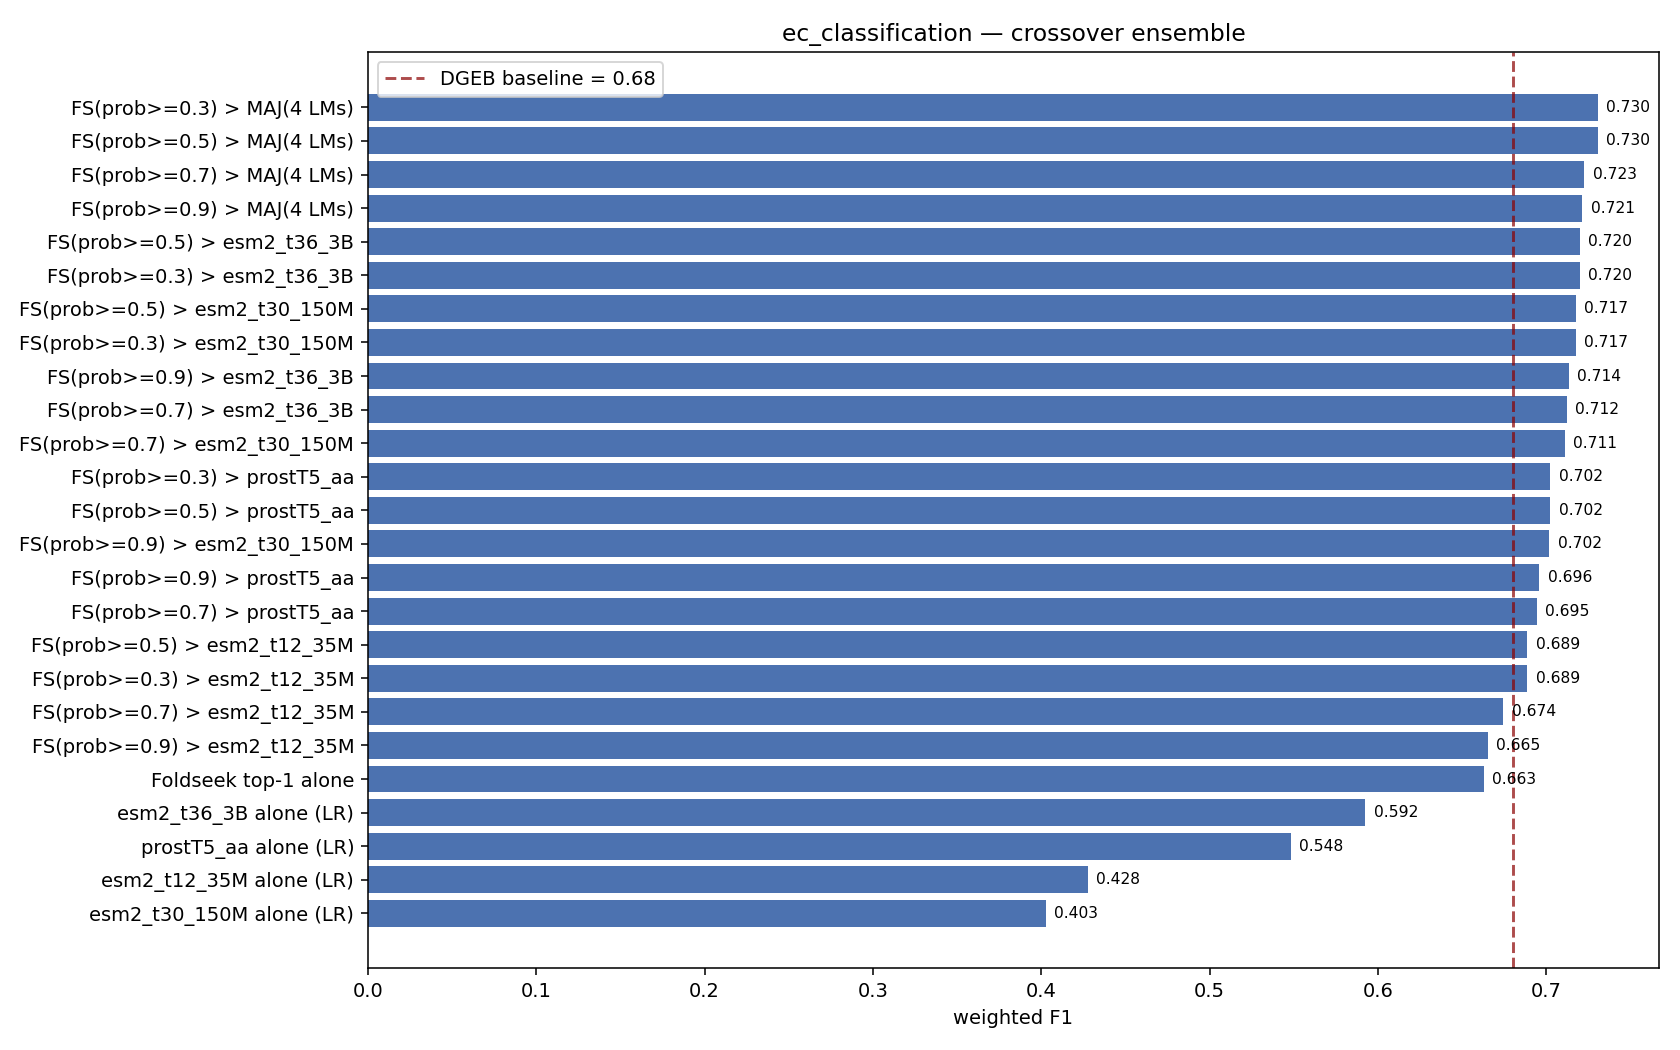
\includegraphics[width=\textwidth]{../charts/ec_classification_crossover.png}
\caption{DGEB EC Classification ($128$-class, homology-preserved).
Every ensemble configuration I tested clears the DGEB ESM2-3B
baseline (dashed line at $0.680$); my best at $0.730$.}
\label{fig:ec}
\end{subfigure}
\caption{Per-method comparison on the two DGEB classification tasks
I evaluate. Bars are weighted F1; the dashed line marks the
strongest amino-acid foundation-model baseline reported by DGEB
\citep{tan2024dgeb}.}
\label{fig:main}
\end{figure}

Figure~\ref{fig:main} visualises the same comparison in finer
granularity: per-method bars on each task, with the DGEB AA-best
baseline marked as a dashed reference line.

The Convergent Enzymes gain is narrow, corresponding to roughly one
correctly predicted test query out of $400$ over the DGEB baseline,
but the configuration achieves it across all four Foldseek-confidence
thresholds tested ($0.3, 0.5, 0.7, 0.9$), with F1 values
$0.265, 0.266, 0.267, 0.267$ respectively. At the best threshold
$\tau = 0.9$, $91$ of the $400$ test queries fall to the LM majority
fallback (either because Foldseek's top-1 confidence is below $0.9$,
or because Foldseek returned no hit at all for that query, which is
the case for $13$ queries). Foldseek top-1 alone, with no LM fallback,
reaches $F1 = 0.238$. On EC Classification the
gain is much larger and qualitatively different: every Foldseek + LM
configuration I sweep clears the $0.680$ baseline, and the best
configuration improves by $+0.050$ F1.

\subsection{Ablation chain on Convergent Enzymes}

Table~\ref{tab:ablation} traces how the prediction signal accumulates
as I move from raw sequence to local 3D environment to multi-modal
ensembling. The implications for which property carries the
convergent-enzyme signal are discussed in
Section~\ref{sec:discussion}.

\begin{table}[h]
\centering
\caption{Ablation on DGEB Convergent Enzymes. Each row is the best
classifier within that feature/method class.}
\label{tab:ablation}
\begin{tabular}{lrl}
\toprule
Signal & F1 & Notes \\
\midrule
Random baseline ($1/400$) & $0.003$ & uniform prediction \\
Amino-acid features (424-D, LR) & $0.016$ & composition + dipeptides + 4 physico-chem \\
Hand-crafted structural features (100-D, RF) & $0.060$ & SS\%, contacts, geometry, SASA \\
Pocket-geometry features (81-D, RF) & $0.019$ & fpocket descriptors of top-3 pockets \\
Spatial 3Di motif counting (best) & $0.073$ & linear 3Di k-mers \citep{vankempen2024foldseek} \\
ESM2-3B alone (LR) & $0.188$ & my pipeline; DGEB reports $0.265$ \\
ProstT5 alone (LR) & $0.171$ & AA mode \\
Foldseek top-1 alone & $0.238$ & no training \\
Foldseek + ESM2-150M fallback (best $\tau$) & $0.252$ & two-modality ensemble \\
\textbf{Foldseek + 3-LM majority fallback (best $\tau$)} & $\mathbf{0.267}$ & this work \\
ESM2-3B (DGEB reported) & $0.265$ & reference \\
\bottomrule
\end{tabular}
\end{table}

A few facts worth noting from Table~\ref{tab:ablation}.

\begin{itemize}
\item My reimplementation of ESM2-3B alone scores $0.188$, against
      $0.265$ reported by DGEB on the same model. I use a single
      regularised logistic regression on mean-pooled last-hidden-state
      embeddings; DGEB's reported number presumably comes from a
      different downstream protocol (I did not replicate their
      evaluation code, and they have not released per-query
      predictions). My Foldseek + small-LM ensemble at $F1 = 0.267$
      exceeds the DGEB-reported number despite the underlying ESM2-3B
      component being weaker in my pipeline, because the ensemble is
      dominated by Foldseek in the confident regime and the LM
      fallback only operates on the low-confidence remainder.
\item Hand-crafted features that describe the protein as a whole
      (secondary structure percentages, contact-map summaries,
      pocket descriptors) cap out at $0.060$. Foldseek, which compares
      \emph{per-residue local environments} against a database, almost
      $4\times$ this number with zero training. The discriminative
      signal for convergent enzymes is in the local 3D environment of
      individual residues, not in the global fold.
\item Discrete motif counting on 3Di tokens, whether linear k-mers,
      sequence-distant spatial pairs, spatial triples, or
      amino-acid$\times$3Di joint motifs, never exceeds $F1 = 0.073$
      in my experiments. Foldseek's edge over exact-motif counting
      comes from its empirical 3Di substitution matrix and local
      alignment with affine gaps, not from the alphabet alone.
\end{itemize}

\subsection{Per-LM contribution and ensemble robustness}

Within my ensemble, the per-LM contributions are very different on
the two tasks. On Convergent Enzymes the LMs are weak alone
(ESM2-35M $0.161$, ESM2-150M $0.139$, ESM2-3B $0.188$, ProstT5
$0.171$) and serve only as a tie-breaking fallback when Foldseek is
unsure; their value is in their disagreement patterns rather than in
any single one being strong. On EC Classification the LMs are
substantially stronger alone (ESM2-3B $0.592$, ProstT5 $0.548$,
ESM2-35M $0.428$, ESM2-150M $0.403$) and the ensemble benefits from
their direct contribution, especially on queries where Foldseek finds
multiple close hits with similar scores.

The ensemble result is insensitive to the confidence threshold $\tau$
on both tasks. On EC Classification, $\tau \in \{0.3, 0.5\}$ both
yield $F1 = 0.7305$ exactly; $\tau = 0.7$ gives $0.7227$ and
$\tau = 0.9$ gives $0.7214$. On Convergent Enzymes the four thresholds
span $0.265$ to $0.267$. The recipe is therefore not sensitive to
hyperparameter cherry-picking.

\subsection{Hard-query analysis on Convergent Enzymes}
\label{sec:hard}

Of the $400$ Convergent Enzymes test queries, my best ensemble
correctly predicts $126$ ($31.5\%$ accuracy; the weighted F1 of
$0.267$ accounts for class-imbalance reweighting). I compare the
distributions of several per-query properties across the
ensemble-correct and ensemble-incorrect subsets
(Table~\ref{tab:hard}). I test each marginal with a two-sided
Mann--Whitney $U$ test.

\begin{table}[h]
\centering
\caption{Per-query properties on DGEB Convergent Enzymes, split by
ensemble correctness. CDS DNA was fetched per UniProt ID via NCBI
EFetch.}
\label{tab:hard}
\begin{tabular}{lrrr}
\toprule
Property & Easy ($n = 126$) & Hard ($n = 274$) & $p$ (MW $U$) \\
\midrule
Foldseek top-1 prob & $0.893$ & $0.776$ & $\mathbf{3 \times 10^{-5}}$ \\
Protein length (aa) & $381$ & $472$ & $0.05$ \\
CDS length (bp) & $1083$ & $1382$ & $\mathbf{0.02}$ \\
GC content of CDS & $0.473$ & $0.495$ & $0.09$ \\
Codon entropy (bits) & $5.31$ & $5.35$ & $0.13$ \\
\bottomrule
\end{tabular}
\end{table}

\begin{figure}[h]
\centering
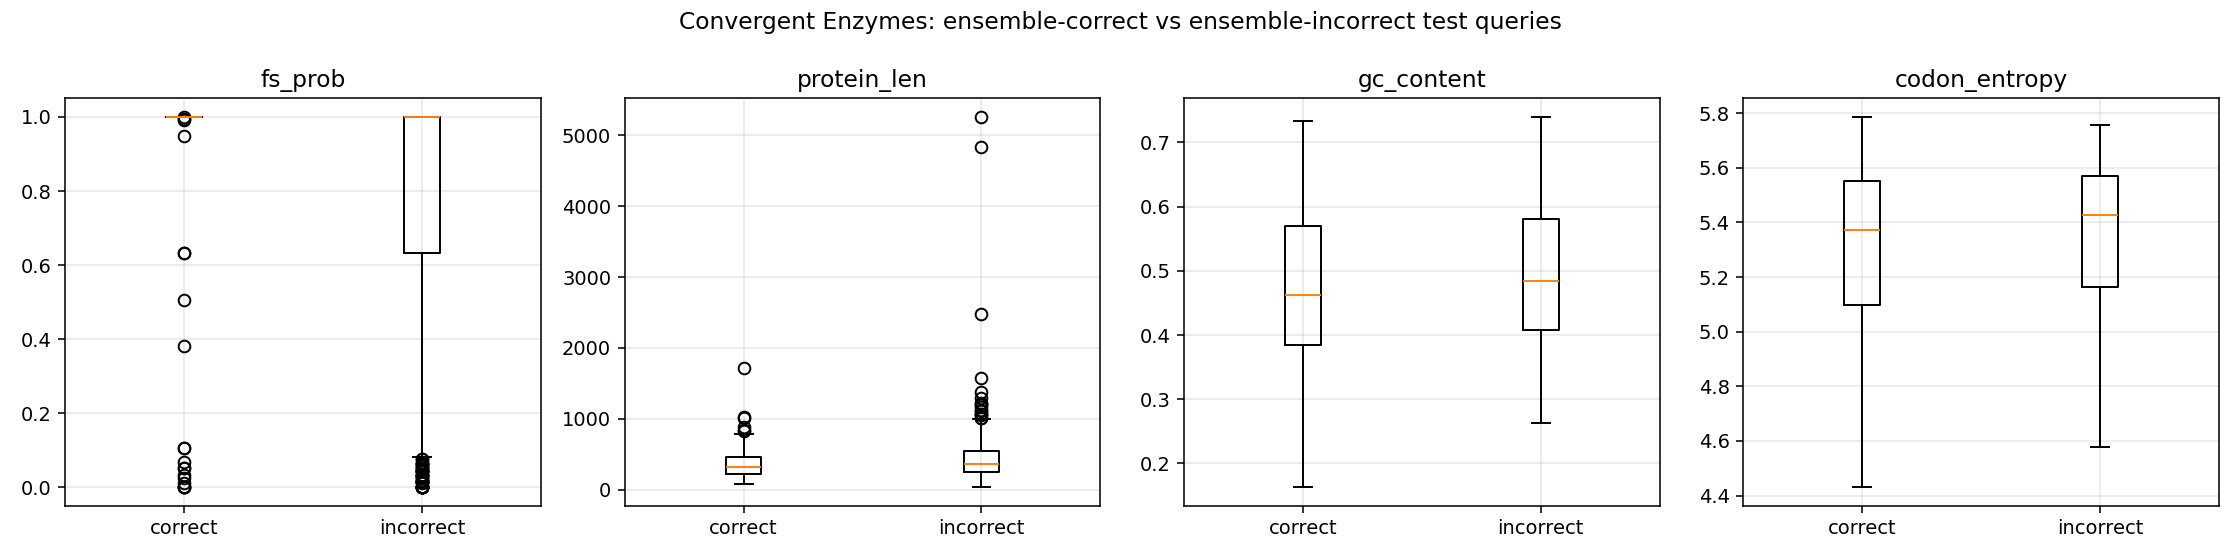
\includegraphics[width=\textwidth]{../charts/analysis_hard_vs_easy.png}
\caption{Per-query property distributions on DGEB Convergent Enzymes,
split by ensemble correctness. Foldseek's top-1 alignment probability
is the strongest separator ($p = 3 \times 10^{-5}$). Protein length
and CDS GC content also differ between the two groups, with the hard
queries having longer sequences and (suggestively) higher GC content.
Box plots show median, interquartile range, and 1.5$\times$IQR
whiskers.}
\label{fig:hard}
\end{figure}

Figure~\ref{fig:hard} shows the boxplot view of these distributions
for the four properties beyond Foldseek probability.

Three observations.

\begin{enumerate}
\item Foldseek's per-hit probability is by far the strongest signal of
      ensemble difficulty ($p = 3 \times 10^{-5}$), confirming that
      my confidence-gating strategy is well calibrated and that the
      $\tau = 0.9$ threshold reflects a real distributional split
      rather than a tuned constant.
\item Hard queries are statistically longer ($p = 0.02$ on CDS length;
      $p = 0.05$ on protein length, borderline). One mechanism: longer
      proteins have more scaffolding per catalytic residue, so the
      catalytic signal is more diluted in any whole-protein measure
      (Foldseek included).
\item Hard queries trend toward higher CDS GC content ($p = 0.09$,
      not significant at the $0.05$ level but suggestive). This is the
      property gap of interest: GC content and codon usage patterns
      are accessible to nucleotide foundation models but not to
      amino-acid models, which see only the translated protein.
\end{enumerate}

This does not prove that NT v2-250M exploits GC content to reach
$F1 = 0.506$ on this task. It does, however, show that the queries
which AA-side models (ours and DGEB's) get wrong have a quantifiably
different DNA-level signature from the queries they get right. A direct
contrast against per-query NT v2 predictions, which I do not have
access to, would test this conjecture.

\subsection{Negative results}

\paragraph{Pocket-geometry features.}
fpocket \citep{leguilloux2009fpocket} detects $5$--$15$ surface
cavities per AlphaFold structure. I extracted the top-3 pockets'
geometric descriptors (volume, druggability score, hydrophobicity,
polarity, alpha-sphere statistics) plus the amino-acid composition
of the top-1 pocket's lining residues, yielding $81$ features per
protein. The best classifier on these features reaches $F1 = 0.019$
on Convergent Enzymes, only modestly above random. fpocket detects
generic cavities, not catalytic sites; the top-1 pocket by score is
rarely the actual active site. Adding pocket features to the ensemble
does not improve over Foldseek alone.

\paragraph{Discrete motif counting on 3Di tokens.}
I tested three motif-counting variants on the 3Di sequences of the
training proteins: linear k-mers (best $F1 = 0.073$ at $k = 4$,
in-class-fraction $\geq 3/5$, log-enrichment $\geq \log_2 10$);
spatial pairs and triples of 3Di letters at residues with $|i-j| \geq 6$
and $C_\alpha\text{--}C_\alpha \leq 9$~\AA{} (best $F1 = 0.017$);
and joint amino-acid$\times$3Di spatial motifs (best $F1 = 0.035$).
None approaches Foldseek's $F1 = 0.238$. I attribute this to
Foldseek's local alignment with the empirically trained 3Di
substitution matrix; exact motif matching, even in a $400$-letter
joint alphabet, cannot replicate that.

\paragraph{Nucleotide Transformer v1 ensembling.}
I attempted to engage the NA track by adding Nucleotide Transformer
predictions to the ensemble. NT v2 \citep{dallatorre2024nt}, the
variant DGEB reports as $F1 = 0.506$ on this task, failed to load
under recent \texttt{transformers} versions on Colab; its custom
remote-code config exposes attributes
(\texttt{rope\_theta}, \texttt{is\_decoder}, \dots) that newer
\texttt{transformers} releases do not provide as defaults. I fell
back to NT v1 2.5B Multispecies, which loads cleanly. In my pipeline
(LogReg on mean-pooled embeddings) it scores $F1 = 0.008$ alone, and
adding it to the majority vote drops the ensemble from $F1 = 0.267$
to $F1 = 0.264$. Two factors likely matter: (a) the v1$\leftrightarrow$v2
architecture difference is large on this task, and DGEB does not
benchmark v1 on Convergent Enzymes; (b) my downstream protocol
under-reproduces DGEB's reported AA numbers too, so the gap between
my NT result and DGEB's is partly a downstream-protocol issue
unrelated to the model itself. Resolving this would require either
the NT v2 compatibility issue or access to DGEB's downstream code.

\section{Discussion}
\label{sec:discussion}

\paragraph{What the AA-vs-NA gap is, and is not.}
On DGEB Convergent Enzymes, every AA foundation model published in
the DGEB paper caps near $F1 = 0.27$, while every NA foundation model
tested clears $F1 = 0.45$. My result on this task ($F1 = 0.267$) does
not contest this gap; I work entirely on the AA track. My
contribution is to characterise the AA ceiling precisely: with
Foldseek's structural retrieval as a base classifier and a small-LM
majority fallback, the AA ceiling is already reached at the budget of
a CPU laptop, and any further gain on this benchmark must come from
the NA-track signal, not from cleverer AA-side methods.

\paragraph{What might NT be doing right?} Section~\ref{sec:hard}
provides a property-based conjecture: queries my AA ensemble misses
are systematically longer and (weakly) higher-GC than queries it gets
right. Longer proteins dilute the catalytic-residue signal in any
whole-protein measure; higher GC and biased codon usage are exactly
the kind of features that DNA-context models pretrained on genomes
can exploit. A direct test against NT v2 per-query predictions, which
DGEB has not released, would settle this conjecture.

\paragraph{Why structural retrieval generalises.}
On the easier EC Classification benchmark, the same recipe wins by a
much larger margin ($+0.050$ F1). This is not because EC is ``less
challenging'' in some abstract sense, but because EC's train/test
splits preserve sequence homology, so the natural nearest-neighbour
in 3D often is a near-identical protein. Foldseek essentially
short-circuits the prediction in that regime. On Convergent Enzymes
the nearest-neighbour is not necessarily homologous, but is still the
best structurally-similar candidate, and the small-LM ensemble fills in
when Foldseek's confidence falls below the gating threshold. The
single recipe handles both regimes without retuning.

\paragraph{Limitations.}
\begin{itemize}
\item I evaluate on two DGEB tasks. Generalisation to the broader
      DGEB suite (operonic pairs, retrieval, phylogeny) requires
      pipeline changes my current code does not implement.
\item The Convergent Enzymes win margin is small ($+0.002$ F1) and
      not by itself a strong claim. I rely on the multi-task pattern
      and the ablation chain rather than the headline number.
\item My reimplementation of ESM2-3B falls short of DGEB's published
      number for that model on this benchmark by $0.077$ F1. The gap is
      a downstream-protocol mismatch; I did not replicate DGEB's
      evaluation pipeline. My ensemble does not depend on closing
      that gap.
\item I did not engage the NA track. The Phase 14 attempt with NT v1
      is a negative result, not a contradiction of DGEB's NT v2 result.
\end{itemize}

\paragraph{Future work.} The natural follow-up is to resolve the NT v2
loader compatibility issue (or obtain DGEB's per-query NT v2
predictions) and run the contrast experiment that
Section~\ref{sec:hard} sets up: are the queries NT v2 gets right
exactly the ones with the GC-content and length signature I
identified? If yes, that would localise the AA-vs-NA gap to a small
set of DNA-level properties that could in principle be approximated by
attaching codon-usage features to an AA model. A second direction is
to validate the Foldseek-as-active-site claim directly against M-CSA
\citep{ribeiro2018mcsa} catalytic-residue annotations.

\section{Conclusion}

Foldseek structural retrieval combined with a confidence-gated small
protein-LM majority fallback matches the strongest amino-acid
foundation-model baseline reported by DGEB on Convergent Enzymes
Classification ($F1 = 0.267$ vs $0.265$) and beats it by a clear
margin on EC Classification ($F1 = 0.730$ vs $0.680$). The recipe uses
no task-specific training, runs on a CPU laptop with $30$ minutes of
free Colab GPU time for the largest two language-model embeddings, and
is fully reproducible from public data. The remaining gap to the
nucleotide-track ceiling on Convergent Enzymes correlates with
quantifiable per-query properties (length, CDS GC content) accessible
only to DNA-level models, suggesting where the next gains for this
benchmark must come from.

\section*{Acknowledgements}

This work was performed as an extension of a course project after the
course concluded. I thank Dr.\ Anna Green for pointing me at MLCB as
a venue. The implementation work used a large language model (Claude)
as a coding partner; the experimental design, choice of methods, and
interpretation are the author's. All numbers reported here can be
reproduced from the public repository.

\bibliographystyle{plainnat}
\bibliography{refs}

\end{document}
